\chapter{Medidor de Presión}
Utilizando un sensor de presión $MDX2010DP$ se diseñó e implementó en PCB un circuito un medidor de presión utilizando un amplificador de instrumentación que cumpla con las especificaciones de la Tabla \ref{e4:tab_specs}, alimentado por una única fuente de tensión.

\begin{table}[ht]
\begin{center}
\begin{tabular}{||c|c||c|c|c||}
\hline
Característica				&Símbolo	&Min	&Máx	&Unidades \\
\hline
Tensión de salida mínima	&$V_{min}$	&0		&0		&$V$ \\
Tensión de salida máxima	&$V_{max}$	&3.1	&3.3	&$V$ \\
Tensión de alimentación		&$V_{DC}$	&10		&15		&$V$ \\
\hline
\end{tabular}
\caption{Especificaciones para el diseño del Medidor de Presión}
\label{e4:tab_specs}
\end{center}
\end{table}

\section{Diseño}
\subsection{Sensor de Presión}
A partir de la hoja de datos del MPX2010DP, se tomó en cuenta la información en la Tabla \ref{e4:tab_sensor_specs} para el diseño del medidor de presión.

\begin{table}[ht]
\begin{center}
\begin{tabular}{||c|c||c|c|c|c||}
\hline
Característica				&Símbolo	&Min	&Typ	&Máx	&Unidades \\
\hline
Rango de Presión			&$P_{OP}$	&0		&-		&10		&$V$ \\
Tensión de alimentación		&$V_{DC}$	&0		&10		&16		&$V$ \\
Tope de Escala				&$V_{FSS}$	&24		&25		&26		&$mV$ \\
Sensibilidad				&$\Delta V / \Delta P$ &-&2.5	&-	&$mV/kPa$\\
\hline
\end{tabular}
\caption{Especificaciones del Sensor de Presión}
\label{e4:tab_sensor_specs}
\end{center}
\end{table}

\subsection{Amplificador de Instrumentación}
Para el Amplificador de Instrumentación (A.I.) se utilizó el diseño de dos amplificadores operacionales ilustrado en la Figura \ref{e4:fig_amp_inst}.
Es posible calcular la ganancia del circuito completo observando que el primer bloque del A.I. se trata de un circuito amplificador no inversor, por lo que su ganancia estará dada por la expresión (\ref{e4:eq_A1}) donde $a_1$ es la ganancia a lazo abierto del amplificador operacional U1 y $v_o'$ es su tensión de salida.

\begin{figure}[ht]
\begin{center}
\begin{circuitikz}[american voltages]
\draw
(0,0) node[op amp] (opamp1) {U1}
(6,-0.5) node[op amp] (opamp2) {U2}
(opamp1.-) to[R=$R_1$,*-] ++(-3,0) to ++(0,-2) node[ground]{GND}
(opamp1.+) to[sinusoidal voltage source=$V_1$] ++(0,-3) node[ground]{GND}
(opamp1.-) to ++(0,1) to[R=$R_2$] ++(3,0) to[short,-*] ++(0,-1.5)
(opamp1.out)to[R=$R_3$,-*] (opamp2.-)
(opamp2.+) to[sinusoidal voltage source=$V_2$] ++(0,-2.5) node[ground]{GND}
(opamp2.-) to ++(0,1) to[R=$R_4$] ++(3,0) to[short] ++(0,-1.5) node[right]{$v_{out}$} to (opamp2.out)
;
\end{circuitikz}
\caption{Amplificador de Instrumentación}
\label{e4:fig_amp_inst}
\end{center}
\end{figure}

\begin{equation}
\mathlarger{
A_1 = \frac{v_o'}{V_1} = \left(1+ \frac{R_2}{R_1}\right) \cdot \frac{1}{1 + \frac{1+R_2/R_1}{a_1}}
}
\label{e4:eq_A1}
\end{equation}

Por otro lado, en la segunda sección del A.I. la salida del amplificador operacional U2 puede calcularse aplicando el principio de superposición entre la tensión $v_o'$ y $V_2$:

\begin{equation}
\mathlarger{
v_{out} = V_2 \cdot \left(1 + \frac{R_4}{R_3}\right) \cdot \frac{1}{1 + \frac{1+R_4/R_3}{a_2}} + v_o' \cdot \left(- \frac{R_4}{R_3}\right) \cdot \frac{1}{1 + \frac{1+R_4/R_3}{a_2}}
}
\label{e4:eq_v_out}
\end{equation}

Operando con las expresiones (\ref{e4:eq_A1}) y (\ref{e4:eq_v_out}) se obtiene para la tensión de salida del A.I.

\begin{equation}
\mathlarger{
v_{out} = \left(1 + \frac{R_4}{R_3}\right) \cdot \frac{1}{1 + \frac{1+R_4/R_3}{a_2}} \cdot \left[ V_2 - V_1 \cdot \frac{1+ R_2/R_1}{1+R_3/R_4} \cdot \frac{1}{1 + \frac{1+R_4/R_3}{a_1}} \right]
}
\label{e4:eq_v_out_a_fin}
\end{equation}

Finalmente, considerando que los amplificadores operacionales tienen una ganancia infinita ($a_1 \cap a_2 \rightarrow \infty$) se obtiene la expresión simplificada 

\begin{equation}
\mathlarger{
v_{out} = \left(1 + \frac{R_4}{R_3}\right) \cdot \left[ V_2 - V_1 \cdot \frac{1+ R_2/R_1}{1+R_3/R_4} \right]
}
\label{e4:eq_v_out_a_inf}
\end{equation}

A partir de la expresión (\ref{e4:eq_v_out_a_inf}) se oberva que el A.I. se encuentra balanceado cuando se cumple la condición

\begin{equation}
\mathlarger{
1+\frac{R_2}{R_1} = 1+\frac{R_3}{R_4} \Rightarrow \frac{R_2}{R_1} = \frac{R_3}{R_4}
}
\label{e4:eq_cond_bal}
\end{equation}

Tomando la expresión \eqref{e4:eq_v_out_a_inf} se pueden calcular las ganancias a modo común ($A_{CM}$) y a modo diferencial ($A_{DM}$)

\begin{equation}
\mathlarger{
A_{CM} = 1 - \frac{R_4}{R_3} \cdot \frac{R_2}{R_1}
}
\label{e4:eq_A_cm}
\end{equation}

\begin{equation}
\mathlarger{
A_{DM} = \frac{R_4}{R_3} + \frac{1}{2} \cdot \left(1+ \frac{R_4}{R_3} \cdot \frac{R_2}{R_1}\right)
}
\label{e4:eq_A_dm}
\end{equation}

Cuando se cumple la condición de balance descripta en \eqref{e4:eq_cond_bal} se obtiene que idealmente $A_{CM_B} = 0$ y $A_{DM_B} = 1+R_4/R_3$.

\begin{equation}
\mathlarger{
CMRR=10\log\left(\frac{A_{DM}}{A_{CM}}\right)
}
\end{equation}

\subsection{Selección de Componentes}
Tomando en cuenta los datos de las Tablas \ref{e4:tab_specs} y \ref{e4:tab_sensor_specs}, se busca que $A_{DM_B}$ esté típicamente dada por la expresión \eqref{e4:eq_r4_r3}. Además, se buscó que se cumpla la condición de balance del A.I. y por lo tanto se tomaron $R_1=R_4$ y $R_3 = R_2$.

\begin{equation}
\mathlarger{
1+ \frac{R_4}{R_3}=\frac{\SI{3.2}{\volt}}{\SI{25}{\milli\volt}}= 128 \Rightarrow R_4=127 R_3
}
\label{e4:eq_r4_r3}
\end{equation}
 
\begin{table}[ht]
\begin{center}
\begin{tabular}{||c|c|c||}
\hline
Resistencia	&	Valor &	Tolerancia\\
\hline	
$R_1$	&	$1.5\si{\mega\ohm} + 22\si{\kilo\ohm}$	&	$5\%$\\
$R_2$	&	$12\si{\kilo\ohm}$	&	$5\%$\\
$R_3$	&	$12\si{\kilo\ohm}$	&	$1\%$\\
$R_4$	&	$1.5\si{\mega\ohm} + 22\si{\kilo\ohm}$	&	$1\%$\\
\hline
\end{tabular}
\end{center}
\caption{Valores de las resistencias}
\label{e4:tab_res_vals}
\end{table}

Las tolerancias fueron seleccionadas por motivos analizados más adelante.

Además, como amplificador operacional se utilizó el \textit{LM833} dado que contiene dos amplificadores operacionales dentro del mismo circuito integrado. Esto permite asumir que ambos \textit{opamps} tienen los mismos parámetros de operación: una impedancia de entrada extremadamente alta, ganancia de tensión iguales en ambos, etc.

\newpage
\section{Simulación}

Con los componentes seleccionados en la Tabla \ref{e4:tab_res_vals} se construyó el circuito en \textit{LTspice XVII} de modo que se puedan simular por separado las ganancias en modo común y en modo diferencial como se ilustra en las Figuras \ref{e4:fig_spice_cm_ac}, \ref{e4:fig_spice_cm_dc}, \ref{e4:fig_spice_dm_ac} y \ref{e4:fig_spice_dm_dc}.

Se observa en los resultados del análisis de Montecarlo en las Figuras \ref{e4:fig_spice_cm_dc_mc} y \ref{e4:fig_spice_dm_dc_mc} que la tensión de salida del Modo Común no excede en módulo los $30 \si{\milli\volt}$ y la tensión de salida del Modo Diferencial se encuentra dentro del rango de tensiones de salida buscadas.

\begin{figure}[ht]
\begin{center}
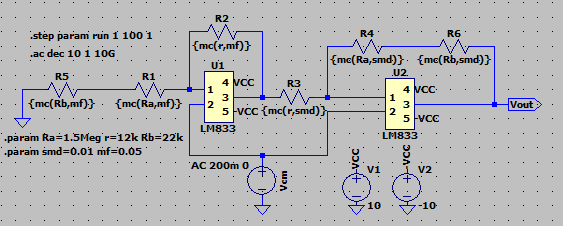
\includegraphics[scale=1]{res/spice/spice_cm_ac_sch.png}
\caption{Esquemático de la simulación en Modo Común en CA}
\label{e4:fig_spice_cm_ac}
\end{center}
\end{figure}

\begin{figure}[ht]
\begin{center}
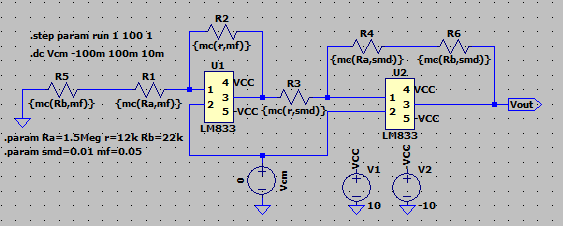
\includegraphics[scale=1]{res/spice/spice_cm_dc_sch.png}
\caption{Esquemático de la simulación en Modo Común en CC}
\label{e4:fig_spice_cm_dc}
\end{center}
\end{figure}

\begin{figure}[ht]
\begin{center}
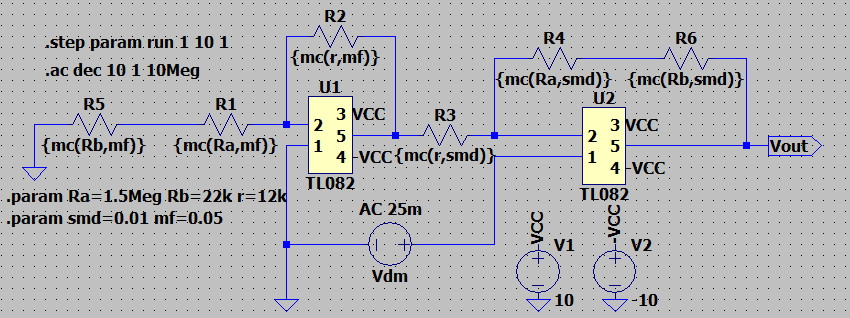
\includegraphics[scale=1]{res/spice/spice_dm_ac_sch.png}
\caption{Esquemático de la simulación en Modo Diferencial en CA}
\label{e4:fig_spice_dm_ac}
\end{center}
\end{figure}

\begin{figure}[ht]
\begin{center}
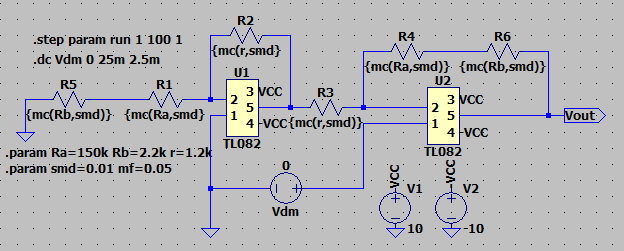
\includegraphics[scale=1]{res/spice/spice_dm_dc_sch.png}
\caption{Esquemático de la simulación en Modo Diferencial en CC}
\label{e4:fig_spice_dm_dc}
\end{center}
\end{figure}

\begin{figure}[ht]
\begin{center}
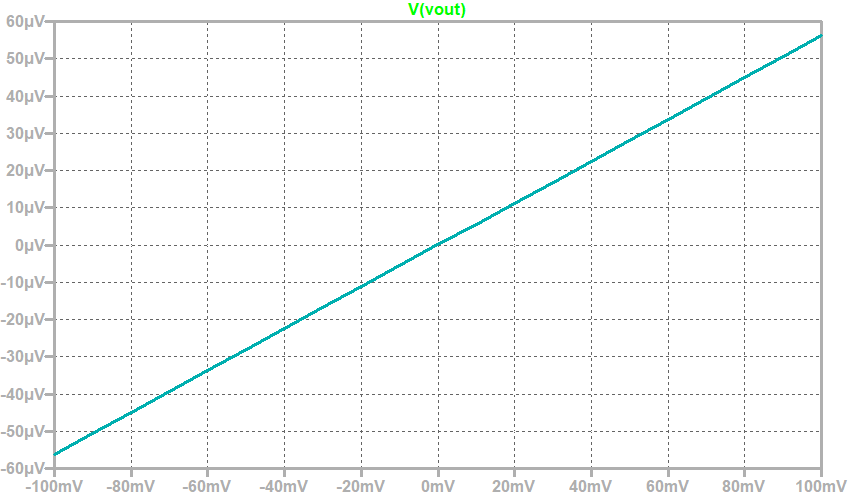
\includegraphics[scale=1]{res/spice/spice_cm_dc.png}
\caption{Resultado de la simulación en Modo Común en CC}
\label{e4:fig_spice_cm_dc_res}
\end{center}
\end{figure}

\begin{figure}[ht]
\begin{center}
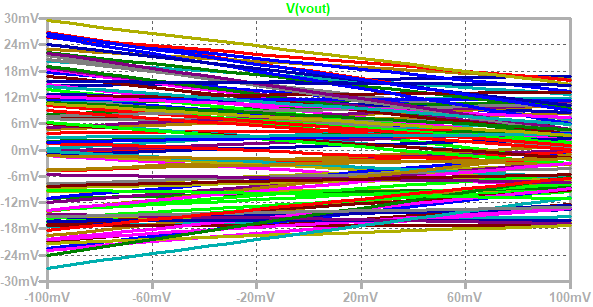
\includegraphics[scale=1]{res/spice/spice_cm_dc_mc.png}
\caption{Resultado del Análisis de Montecarlo en Modo Común en CC}
\label{e4:fig_spice_cm_dc_mc}
\end{center}
\end{figure}

\begin{figure}[ht]
\begin{center}
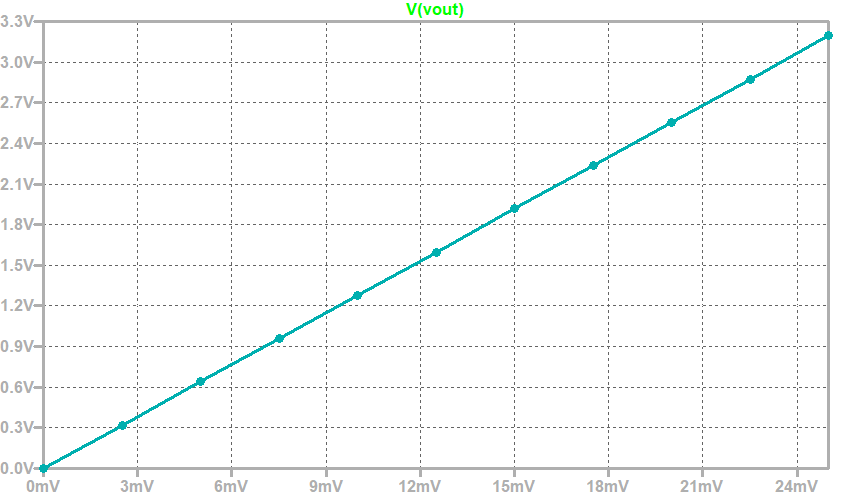
\includegraphics[scale=1]{res/spice/spice_dm_dc.png}
\caption{Resultado de la simulación en Modo Diferencial en CC}
\label{e4:fig_spice_dm_dc_res}
\end{center}
\end{figure}

\begin{figure}[ht]
\begin{center}
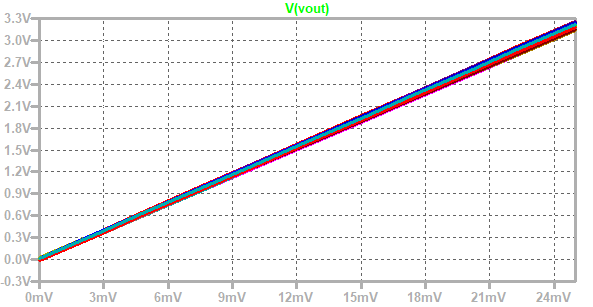
\includegraphics[scale=1]{res/spice/spice_dm_dc_mc.png}
\caption{Resultado del Análisis de Montecarlo en Modo Diferencial en CC}
\label{e4:fig_spice_dm_dc_mc}
\end{center}
\end{figure}

\begin{figure}[ht]
\begin{center}
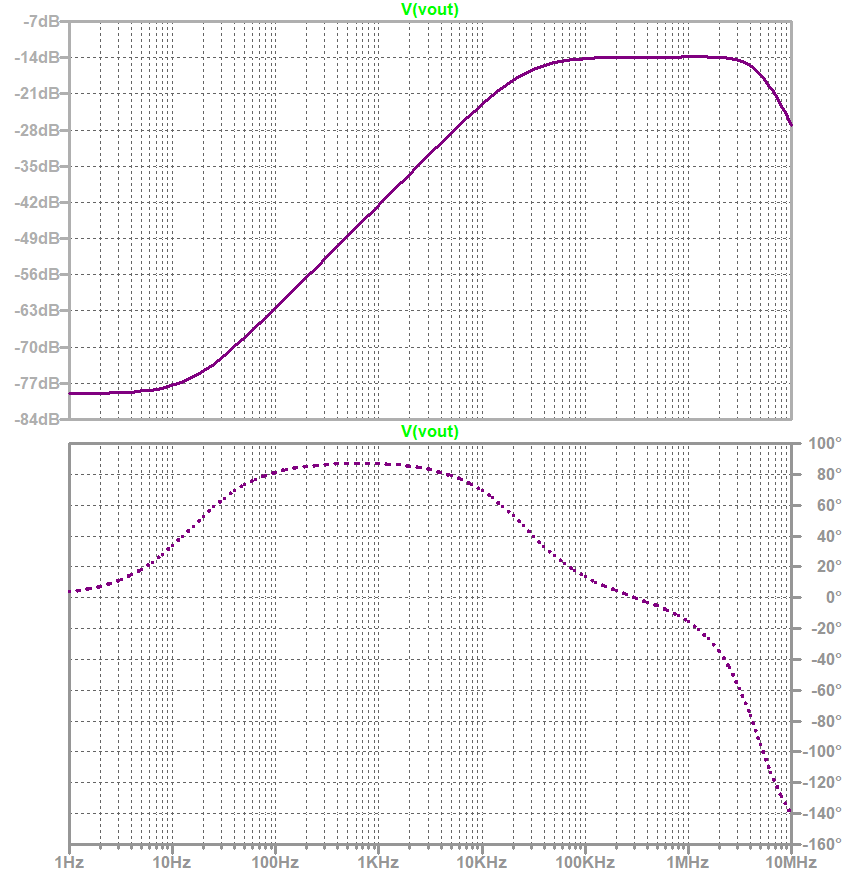
\includegraphics[scale=1]{res/spice/spice_cm_ac_bode.png}
\caption{Resultado de la simulación en Modo Común en AC}
\label{e4:fig_spice_cm_ac_res}
\end{center}
\end{figure}

\begin{figure}[ht]
\begin{center}
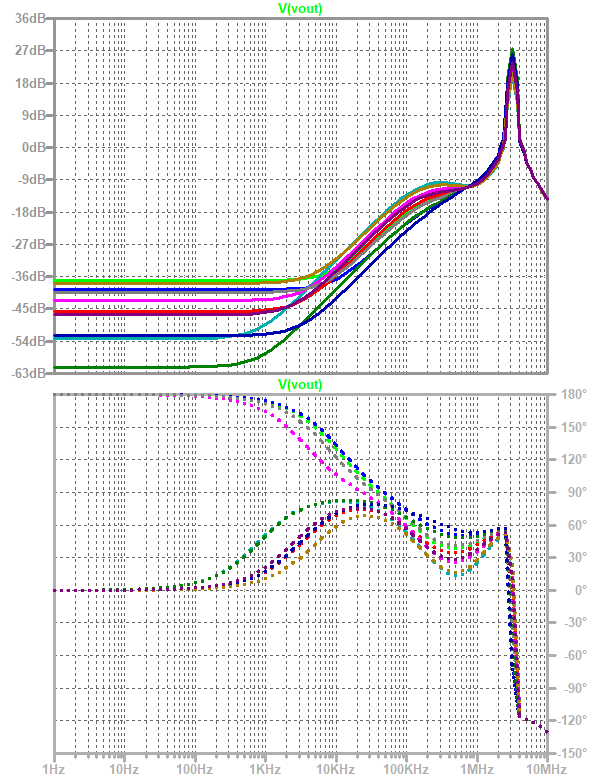
\includegraphics[scale=1]{res/spice/spice_cm_ac_bode_mc.png}
\caption{Resultado del Análisis de Montecarlo en Modo Común en AC}
\label{e4:fig_spice_cm_ac_mc}
\end{center}
\end{figure}

\begin{figure}[ht]
\begin{center}
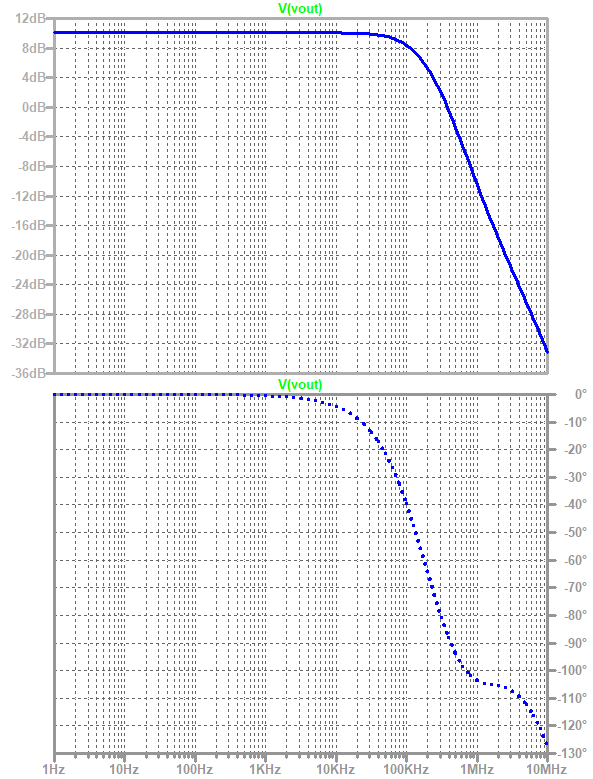
\includegraphics[scale=1]{res/spice/spice_dm_ac_bode.png}
\caption{Resultado de la simulación en Modo Diferencial en AC}
\label{e4:fig_spice_dm_ac_res}
\end{center}
\end{figure}

\begin{figure}[ht]
\begin{center}
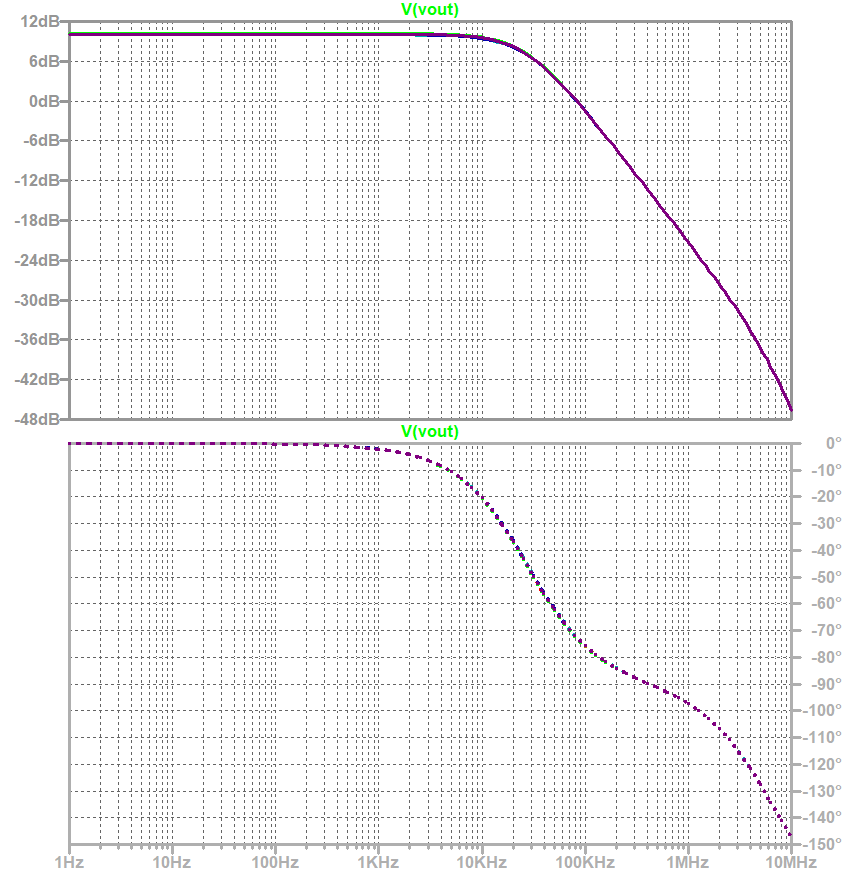
\includegraphics[scale=1]{res/spice/spice_dm_ac_bode_mc.png}
\caption{Resultado del Análisis de Montecarlo en Modo Diferencial en AC}
\label{e4:fig_spice_dm_ac_mc}
\end{center}
\end{figure}

\newpage

\section{Construcción del PCB}

\begin{figure}[ht]
\begin{center}
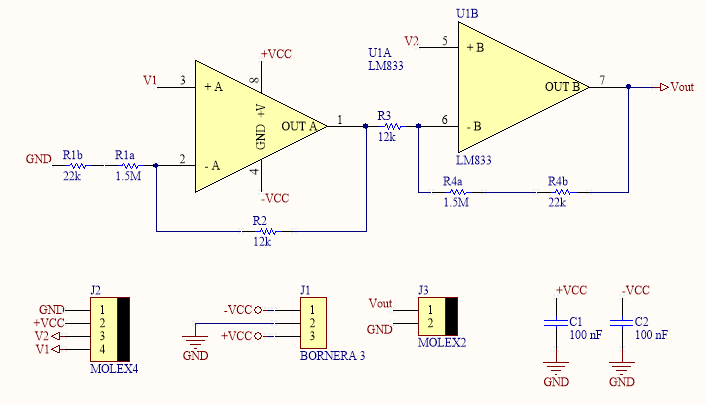
\includegraphics[height=10cm]{res/altium/sch.png}
\caption{Esquemático del Amplificador de Instrumentación}
\label{e4:fig_pcb_sch}
\end{center}
\end{figure}

\begin{figure}[ht]
\begin{center}
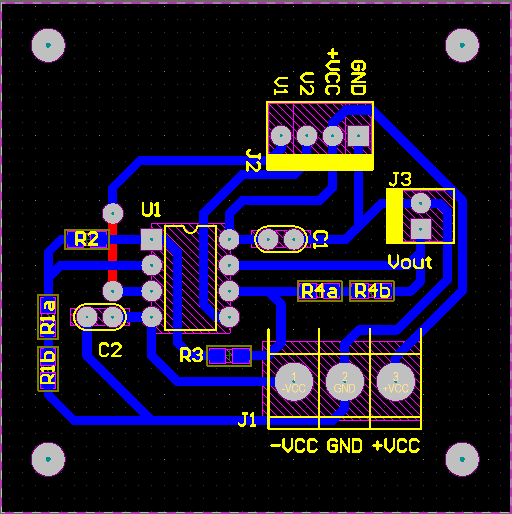
\includegraphics[height=10cm]{res/altium/pcb.png}
\caption{Routeado del PCB del Amplificador de Instrumentación}
\label{e4:fig_pcb_route}
\end{center}
\end{figure}

\section{Mediciones}
Se utilizaron generadores de onda para medir la ganancia del Amplificador de Instrumentación en modo diferencial y en modo común. A partir de estas mediciones se calculó el rechazo a modo común.